\documentclass{standalone}

\usepackage{tikz}

\newlength{\len}
\setlength{\len}{1mm}

\begin{document}

\begin{tikzpicture}[x=\len, y=\len]
  \draw (0, 0) node(a){\includegraphics[width=100\len, draft]{src/lc3pi-spectrum-skim-raw.pdf}};

  \draw (a.north west) node[rotate=90, anchor=north east]{Candidates / $5$ MeV/$c^2$\phantom{00}};

  \draw (a.south) node[anchor=south]{$m(\Lambda_c^+\pi^+\pi^-\pi^-)$};

  \draw (a.south east) node[anchor=south east]{[GeV/$c^2$]};

  \draw (12, 33) node[anchor=north west](LHCb){LHCb Unofficial};
  \draw (LHCb.south east) node[anchor=north east]{9 fb$^{-1}$};
  \draw (5, 25) node[anchor=north west]{
    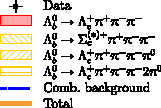
\includegraphics[width=35\len]{src/lc3pi-model-legend-LOL}
  };

\end{tikzpicture}

\end{document}
